\documentclass{homework}
\usepackage{setspace}
\onehalfspacing
\usepackage{float}
\usepackage{needspace}
% \Needspace{10\baselineskip}  % adjust based on expected box height
\usepackage{placeins}
\FloatBarrier
\usepackage{fvextra}
\usepackage{minted} % for code highlighting
\usepackage[most]{tcolorbox}
\tcbuselibrary{listings, minted, breakable}


\author{Shivam Kumar}
\class{Roll. No.: 22CE01046}
\date{\today}
\title{Assignment-1 (CAD Laboratory)}
% \address{CAD Laboratory}

% ---------- Colors ----------
\definecolor{pbheader}{RGB}{240,240,240}   % header background
\definecolor{framecol}{RGB}{190,190,190}   % frame color  
\definecolor{solcol}{RGB}{230,240,250}
\definecolor{mybg}{RGB}{245,245,230}

% ---------- Solution environment ----------
\newtcolorbox{solution}{
  enhanced,
  breakable,
  sharp corners=all,
  colframe=framecol,
  colback=solcol,
  left=6pt, right=6pt, top=6pt, bottom=6pt,
  boxrule=0.5pt,
  before skip=6pt,
  after skip=12pt,
  fonttitle=\bfseries,
  borderline west={2pt}{0pt}{pbheader}
}

% % % Configure minted for Julia
\setminted[julia]{
    linenos,          % show line numbers
    breaklines,      % wrap long lines
    breakanywhere,
    breakautoindent=true,
    fontsize=\small,  % smaller font
    bgcolor=mybg,     % light gray background
    frame=none,          % frame around code
    numbersep=5pt,        % space between line numbers and code
    xleftmargin=10pt      % left margin
}

\graphicspath{{./media/}}

\begin{document} \maketitle

\rule{\linewidth}{0.4pt} 
    \textbf{Package:} Plots.jl; LaTeXStrings.jl; CalculusWithJulia.jl, PythonPlot. \\
\rule{\linewidth}{0.4pt}  % draws a thin horizontal line across the page

\section{Plots.jl with pythonplot()}
\begin{itemize}
    \item Pythonplot() backend: Switches the plotting engine to Matplotlib (via Python), giving access to Matplotlib’s familiar style and fine-grained control.
    \item Create 2D and 3D plots (line, scatter, contour, surface, etc.).
    \item Customize plots with labels, legends, colors, and styles.
\end{itemize}

\section{LaTeXStrings.jl}
\begin{itemize}
    \item Allows you to use LaTeX math notation directly in Julia strings.
    \item Write axis labels, titles, and annotations in LaTeX form, e.g. xlabel=L"x", ylabel=L"\(\sin(x)\)".
    \item Ensure mathematical expressions in plots look professional and consistent with academic writing.
\end{itemize}

\section{CalculusWithJulia.jl}
\begin{itemize}
    \item CalculusWithJulia.jl allows fast, accurate, and interactive computation of derivatives, integrals, and limits, making calculus easier to understand and apply while reducing manual errors.
\end{itemize}

\section{Proble Statement}
\begin{minted}{julia}
    # Import the necessary packages.
    import Pkg;
    Pkg.add(["Plots", "LaTeXStrings", "CalculusWithJulia","PyPlot"])
\end{minted}

\question  Consider that the height of a hill is described by the given scalar field as 
\[
h(x,y) = 200 - x^2 - 2y^2 
\]
 (a) Plot the given scalar field as both a three-dimensional (3D) surface plot and a two-dimensional (2D)
 contour plot using Julia. (you may use the package \textbf{Plots.jl} for plotting).\\
 (b) Plot the gradient of the scalar field using the automatic gradient calculation tool available in Julia
 (you may use the package called \textbf{CalculusWithJulia.jl}).\\
 (c) Determine the gradient vector and plot the obtained gradient vector field (you may use the package
 called \textbf{Plots.jl} or \textbf{CalculusWithJulia.jl}).

\begin{solution}
    \textbf{Solution: 1}
    (a) Two-dimensional (2D) contour plot.
    \begin{minted}{julia}
    using Plots; pythonplot()
    using LaTeXStrings
    
    # Write the function.
    f(x, y) = 200 - x^2 - 2y^2
    
    # Define range of x and y.
    x_range = range(-20, 20, length=100)
    y_range = range(-20, 20, length=100)
    
    # Store the z value at every possible combination of x and y in the array.
    z = [f(x,y) for y in y_range, x in x_range]

    # Now we have a value of x, y and z

    #generating 2D contour graph
    contour(x_range, y_range, z, levels=10,color=:turbo, clabels=true, cbar=true, lw=2)
    title!(L"2D Contour Plot of $200 - x^2 - 2y^2$")
    xlabel!(L"x")
    ylabel!(L"y")
    \end{minted}
    
    \begin{itemize}
        \item levels=10 → Draws 10 contour levels (lines of equal function value).
        \item color=:turbo → Uses the Turbo colormap (a vivid rainbow‑like gradient).
        \item clabels=true → Adds labels directly on the contour lines to show their values.
        \item cbar=true → Displays a color bar on the side, mapping colors to function values.
        \item lw=2 → Sets the line width of the contour lines to 2 (thicker lines for clarity).
        \item Output $\rightarrow$ Figure -~\ref{fig:contour}
    \end{itemize}
    
    % \img<wheel>[0.5]{Cipher wheels.}{2Dcontour_plot.png}
    \begin{figure}[H]
        \centering
        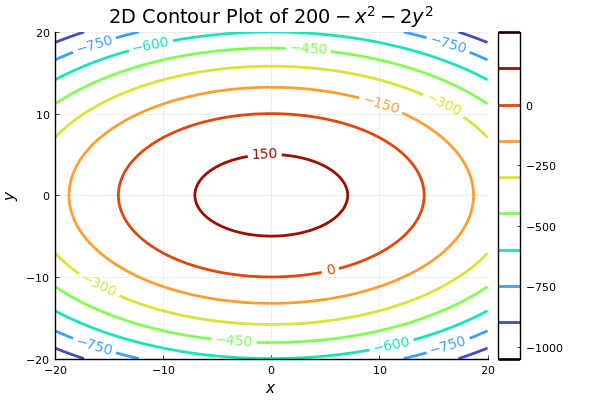
\includegraphics[width=0.5\linewidth]{2Dcontour_plot.png}
        \caption{2D Contour Plot of $200 - x^2 - 2y^2$}
        \label{fig:contour}
    \end{figure}

    
    \textbf{Solution: 1}(a) Three-dimensional (3D) surface plot
    \begin{minted}{julia}
    # 3D Surface Plot
    surface(x_range, y_range, z, title="3D Surface Plot of", xlabel="x", ylabel="y", zlabel="h(x,y)")
    \end{minted}
    
    \begin{itemize}
      \item Output $\rightarrow$ Figure -~\ref{fig:3Dcoutour}
    \end{itemize}
    
    \begin{figure}[H]
      \centering
      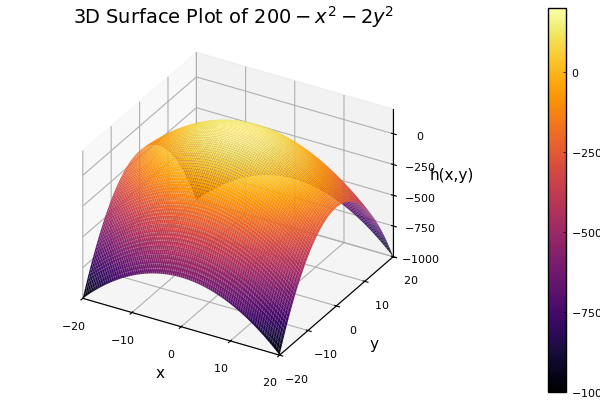
\includegraphics[width=0.5\linewidth]{media/3Dsurface_plot.png}
      \caption{3D Surface Plot of $200 - x^2 - 2y^2$}
      \label{fig:3Dcoutour}
    \end{figure}
    
    \textbf{Solution: 1}
    (b)  Plot the gradient of the scalar field.
    \begin{minted}{julia}
    using CalculusWithJulia

    # Define the function as a single-argument vector function
    f(v) = 200 - v[1]^2 - 2*v[2]^2
    # Get the gradient function using CalculusWithJulia
    grad_h = gradient(f)

    # Store the possible x and y coordinates.
    x_coords = [x for x in x_range for y in y_range]
    y_coords = [y for x in x_range for y in y_range]

    # Calculate the gradient vectors at each point (x, y)
    vectors = [grad_h([x, y]) for x in x_range for y in y_range]

    # Split the vector into the component.
    u = getindex.(vectors,1)
    v = getindex.(vectors,2)

    # quiver plot (a vector field plot)
    # Plot the vector field
    quiver(x_coords, y_coords, quiver=(u, v),arrowsize=0.01,
    title="Gradient Vector Field", xlabel="x", ylabel="y")
    \end{minted}
    
    \begin{itemize}
        \item Output $\rightarrow$ Figure -~\ref{fig:autogradient}
    \end{itemize}
    
    \begin{figure}[H]
        \centering
        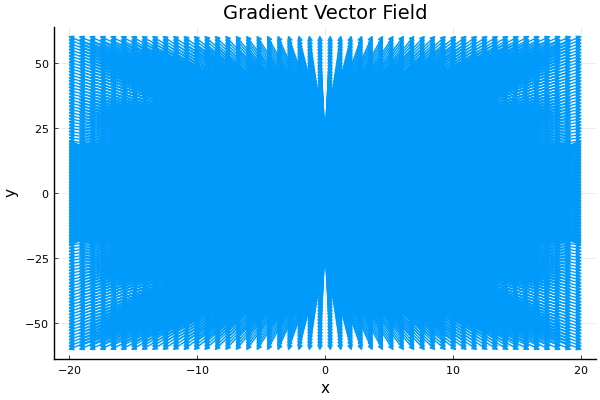
\includegraphics[width=0.5\linewidth]{media/gradientauto.png}
        \caption{Gradient Vector Field}
        \label{fig:autogradient}
    \end{figure} 
    
    \textbf{Solution: 1}
    (c)  Plot the gradient of the scalar field.
    \begin{minted}{julia}
    # Define the components of the gradient vector field
    fx(x, y) = -2x
    fy(x, y) = -4y
    u_coords = [fx(x,y) for x in x_range for y in y_range]
    v_coords = [fy(x,y) for x in x_range for y in y_range]
    
    # Plot the quiver plot using the calculated components
    quiver(x_coords, y_coords, quiver=(u_coords, v_coords),arrowsize=0.01,
    title="Gradient Vector Field (Calculated)", xlabel="x", ylabel="y")
    \end{minted}
    
    \begin{itemize}
        \item Output $\rightarrow$ Figure -~\ref{fig:calgradient}
    \end{itemize}
    
    \begin{figure}[H]
        \centering
        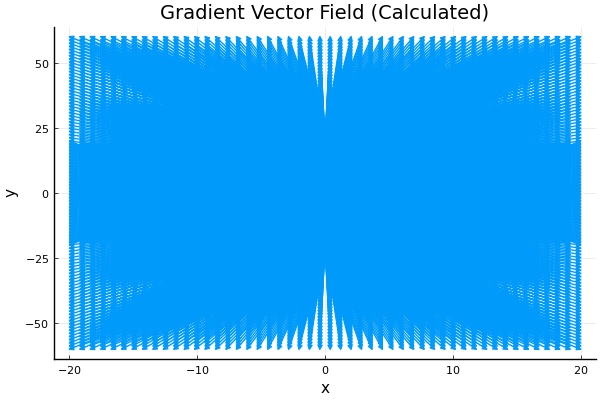
\includegraphics[width=0.5\linewidth]{media/gradientcal.png}
        \caption{Gradient Vector Field (Calculated)}
        \label{fig:calgradient}
    \end{figure}
\end{solution}

\question  Consider a cyclone in the northern hemisphere described by the velocity vector field of the wind
\[
   v(x,y) = xe_1 - y^2e_2
\]
where x and y are the coordinates in the horizontal plane, and e1 and e2 are unit vectors in the x- and
y-directions, respectively.\\
(a) Plot the given vector field in Julia. (you may use the package called \textbf{Plots.jl} or \textbf{CalculusWithJulia.jl}).\\
(b) Plot the divergence of the vector field using automatic divergence calculation available in the Julia package called \textbf{CalculusWithJulia.jl}. Also, determine the divergence using the detailed calculation and plot the same. Compare both plots and verify the results.\\
(c) Determine the curl of the vector field using automatic curl calculation available in the Julia package \textbf{CalculusWithJulia.jl}. Also, determine the curl using detailed calculation and plot the same. Compare both plots and verify the results.

\begin{solution}
    \textbf{Solution: 2}
    (a)  Ploting the vector field.
    \begin{minted}{julia}
    using Plots

    # Define the vector field function
    v1(x, y) = (x, -y^2)

    # Define the x and y range.
    x_range = -2.0:0.2:2.0
    y_range = -2.0:0.2:2.0

    # Define the cordinate of x and y.
    x_coords = [x for x in x_range for y in y_range]
    y_coords = [y for x in x_range for y in y_range]

    # Calculate the components of the vectors at each point
    u_coords = [v1(x, y)[1] for x in x_range for y in y_range]
    v_coords = [v1(x, y)[2] for x in x_range for y in y_range]

    # Create the quiver plot
    quiver(x_coords, y_coords, quiver=(u_coords, v_coords), arrowsize=0.01, legend=false, title=L"Vector Field $v(x,y) =  xe_1 -y^2e_2$", xlabel="x", ylabel="y")
    \end{minted}
    
    \begin{itemize}
        \item Output $\rightarrow$ Figure -~\ref{fig:vectorfield}
    \end{itemize}
    
    \begin{figure}[H]
        \centering
        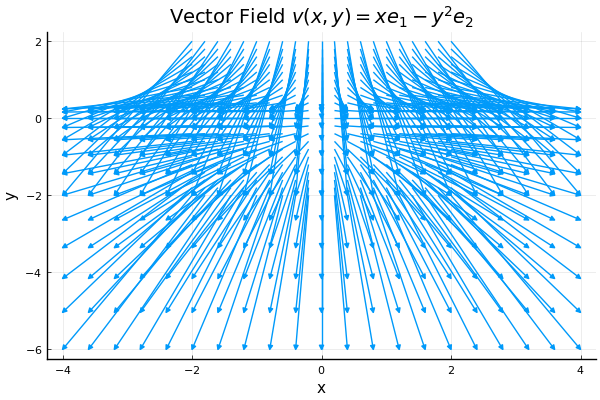
\includegraphics[width=0.5\linewidth]{media/vectorfield.png}
        \caption{Vector Field $v(x,y) = xe_1 - y^2e_2$}
        \label{fig:vectorfield}
    \end{figure}
    
    \textbf{Solution: 2}
    (b)  Divergence calculation using  automatic divergence calculation and detailed calculation
    \begin{minted}{julia}
    using CalculusWithJulia

    # Define the vector field as a function
    v1(x, y) = [x, -y^2]
    v_vec(xy) = v1(xy[1], xy[2])

    # --- Automatic Divergence Calculation ---
    # The divergence function `divergence(f)` will return a new function representing the divergence
    div_auto = divergence(v_vec)

    # Calculate the values of the divergence on the grid
    Z_auto = [div_auto([x, y]) for y in y_range, x in x_range]

    # Plot the automatic divergence
    p1 = heatmap(x_range, y_range, Z_auto, aspect_ratio=:equal, title="Automatic Divergence", xlabel="x",  ylabel="y", colorbar_title="div(v)")
    
    # --- Detailed (Manual) Divergence Calculation ---
    # Define the function for the manual calculation
    div_manual(x, y) = 1 - 2y

    # Calculate the values of the manual divergence on the grid
    Z_manual = [div_manual(x, y) for y in y_range, x in x_range]   
    \end{minted}
    \begin{minted}{julia}   
     # Plot the manual divergence
    p2 = heatmap(x_range, y_range, Z_manual, aspect_ratio=:equal, title="Detailed Divergence", xlabel="x",  ylabel="y", colorbar_title="div(v)")
    
    # Combine plots for comparison
    plot(p1, p2, layout=(1, 2), size=(900, 400))
    \end{minted}
    
    \begin{itemize}
        \item Output $\rightarrow$ Figure -~\ref{fig:divercalvsauto}
    \end{itemize}
    
    \begin{figure}[H]
        \centering
        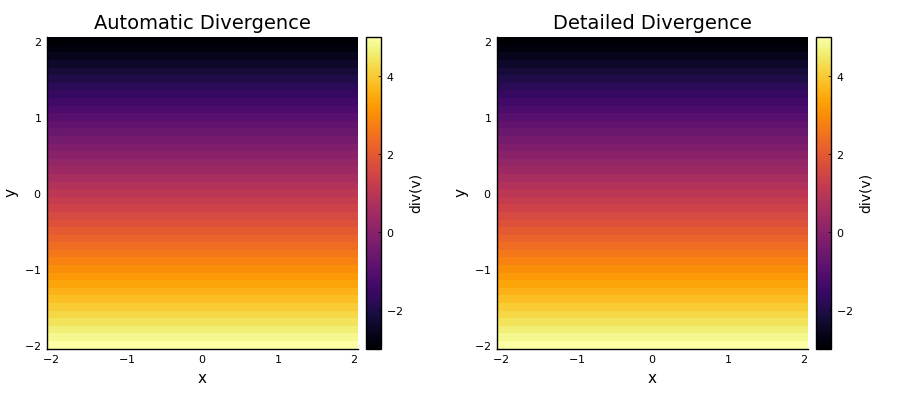
\includegraphics[width=0.5\linewidth]{media/divercalvsauto.png}
        \caption{Divergence using automatic divergence calculation and detailed calculation}
        \label{fig:divercalvsauto}
    \end{figure}
    
    \textbf{Solution: 2}
    (c)  Curl calculation using  automatic curl calculation and detailed calculation.
    \begin{minted}{julia}  
    # --- Automatic Curl Calculation ---
    # The curl function `curl(f)` returns a new function that returns a scalar
    curl_auto = curl(v_vec)

    # Calculate the values of the automatic curl on the grid.
    Z_auto_curl = [curl_auto([x, y]) for y in y_range, x in x_range]

    # Plot the automatic curl
    p3 = heatmap(x_range, y_range, Z_auto_curl, aspect_ratio=:equal,  title="Automatic Curl", xlabel="x", ylabel="y", colorbar_title="curl(v)")
    
    # --- Detailed (Manual) Curl Calculation ---
    # Define the function for the manual calculation
    # The curl is dQ/dx - dP/dy = 0 - 0 = 0.
    curl_manual(x, y) = 0.0   

    # Calculate the values of the manual curl on the grid
    Z_manual_curl = [curl_manual(x, y) for y in y_range, x in x_range]
    
    # Plot the manual curl
    p4 = heatmap(x_range, y_range, Z_manual_curl, aspect_ratio=:equal, title="Detailed Curl", xlabel="x", ylabel="y", colorbar_title="curl(v)")
    \end{minted}
    \begin{minted}{julia}  
    # Combine plots for comparison
    plot(p3, p4, layout=(1, 2), size=(900, 400))
    \end{minted}
    
    \begin{itemize}
        \item Output $\rightarrow$ Figure -~\ref{fig:curlcalvsauto}
    \end{itemize}
    
    \begin{figure}[H]
        \centering
        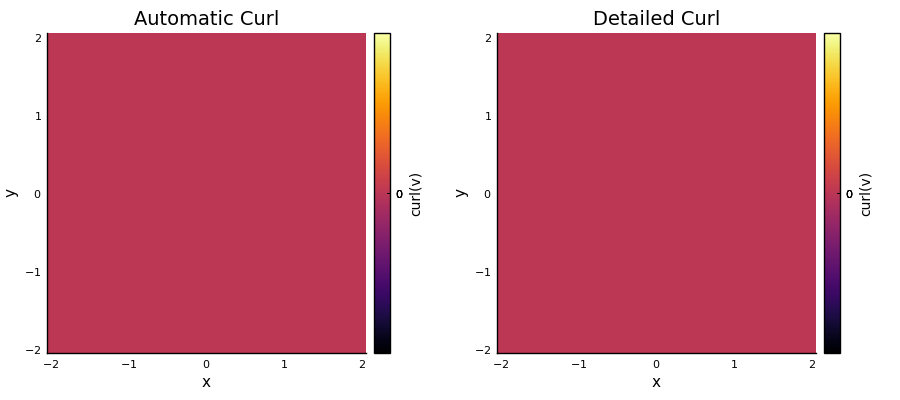
\includegraphics[width=0.5\linewidth]{media/curlcalvsauto.png}
        \caption{Curl using  automatic curl calculation and detailed calculation.}
        \label{fig:curlcalvsauto}
    \end{figure} 
\end{solution}

\question  Consider that the velocity of water particles in a river is described by the vector field
\[
f = e^x y^2 \mathbf{e}_1 + (x + 2y) \mathbf{e}_2
\]

(a) Plot the given vector field in Julia. (you may use the package called \textbf{Plots.jl} or \textbf{CalculusWithJulia.jl}).\\
(b) Plot the divergence of the vector field using automatic divergence calculation available in the Julia package called \textbf{CalculusWithJulia.jl}. Also, determine the divergence using the detailed calculation and plot the same. Compare both plots and verify the results.\\
(c) Determine the curl of the vector field using automatic curl calculation available in the Julia package \textbf{CalculusWithJulia.jl}. Also, determine the curl using detailed calculation and plot the same. Compare both plots and verify the results.

\begin{solution}
    \textbf{Solution: 3}
    (a)  Ploting the vector field.
    \begin{minted}{julia}
    using Plots

    # Define the vector field function
    f(x, y) = (x * y^2, x + 2y)
    
    # Define the grid for the plot
    x_range = -2.0:0.2:2.0
    y_range = -2.0:0.2:2.0

    # Define the cordinate of x and y.
    x_coords = [x for x in x_range for y in y_range]
    y_coords = [y for x in x_range for y in y_range]
    \end{minted}
    \begin{minted}{julia}    
    # Calculate the components of the vectors at each point
    u_coords = [f(x, y)[1] for x in x_range for y in y_range]
    v_coords = [f(x, y)[2] for x in x_range for y in y_range]

    # Create the quiver plot
    plot_vf = quiver(x_coords, y_coords, quiver=(u_coords, v_coords), 
    arrowsize=0.3, 
    legend=false, 
    title="Vector Field f(x,y)",
    xlabel="x",
    ylabel="y")
    \end{minted}
    
    \begin{itemize}
        \item Output $\rightarrow$ Figure -~\ref{fig:vectorfield-2}
    \end{itemize}
    
    \begin{figure}[H]
        \centering
        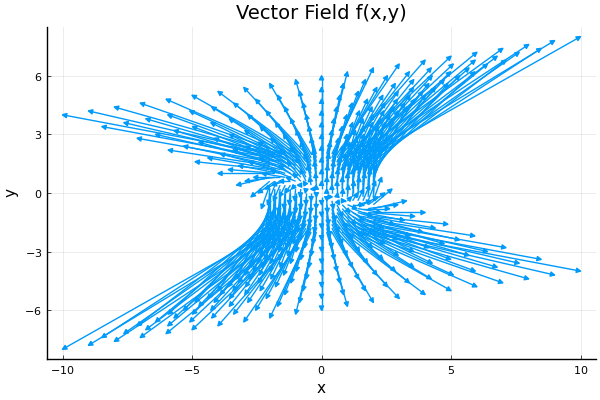
\includegraphics[width=0.5\linewidth]{media/vectorfield-2.png}
        \caption{Vector Field $f = e^xy^2e_1 + (x + 2y)e_2 $}
        \label{fig:vectorfield-2}
    \end{figure}
    
    \textbf{Solution: 3}
    (b)  Divergence calculation using automatic divergence calculation and detailed calculation.
    \begin{minted}{julia}
    using CalculusWithJulia

    # Corrected function definition to take a single vector `p`
    v1(x,y) = [e^x*y^2, x+2*y]
    f(p) = v1(p[1], p[2])
    
    # --- Automatic Divergence Calculation ---
    # The divergence function now works correctly on `f`
    div_auto = divergence(f)  
    \end{minted}
    \begin{minted}{julia}
    # Calculate the values of the automatic divergence on the grid.
    # Note: We now pass a single vector `[x, y]` to `div_auto`.
    Z_auto_div = [div_auto([x, y]) for y in y_range, x in x_range]
    
    # Plot the automatic divergence
    p1 = heatmap(x_range, y_range, Z_auto_div, aspect_ratio=:equal, title="Automatic Divergence", xlabel="x", ylabel="y", colorbar_title="div(f)")

    # --- Detailed (Manual) Divergence Calculation ---
    # This part does not need correction as it is not using the automatic method
    div_manual(x, y) = y^2*e^x + 2
    Z_manual_div = [div_manual(x, y) for y in y_range, x in x_range]
    
    # Plot the manual divergence
    p2 = heatmap(x_range, y_range, Z_manual_div, aspect_ratio=:equal, title="Detailed Divergence", xlabel="x", ylabel="y", colorbar_title="div(f)")

    # Combine and display plots for comparison
    plot(p1, p2, layout=(1, 2), size=(900, 400))
    \end{minted}
    
    \begin{itemize}
        \item Output $\rightarrow$ Figure -~\ref{fig:divegencecalvsauto-2}
    \end{itemize}
    
    \begin{figure}[H]
        \centering
        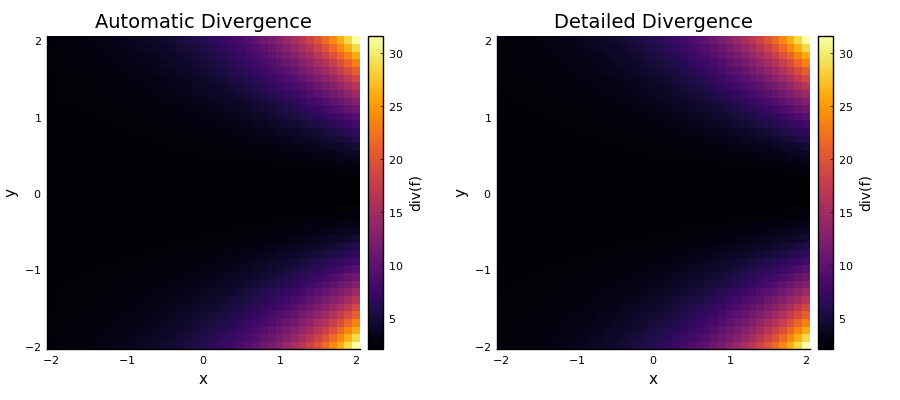
\includegraphics[width=0.5\linewidth]{media/divegencecalvsauto-2.png}
        \caption{Plots of  automatic and manual divergence calculation.}
        \label{fig:divegencecalvsauto-2}
    \end{figure}
    
    \textbf{Solution: 3}
    (c)  Curl calculation using automatic curl calculation and detailed calculation.
    \begin{minted}{julia}
    # Use the same corrected function definition from part (b)
    f(p) = [e^p[1] * p[2]^2, p[1] + 2 * p[2]]
    
    # --- Automatic Curl Calculation ---
    # The curl function now works correctly on `f`
    curl_auto = curl(f)
    \end{minted}
    \begin{minted}{julia}
    # Calculate the values of the automatic curl on the grid.
    Z_auto_curl = [curl_auto([x, y]) for y in y_range, x in x_range]
    
    # Plot the automatic curl
    p3 = heatmap(x_range, y_range, Z_auto_curl, aspect_ratio=:equal, title="Automatic Curl", xlabel="x", ylabel="y", colorbar_title="curl(f)")
    
    # --- Detailed (Manual) Curl Calculation ---
    # This part does not need correction
    curl_manual(x, y) = 1 - 2*e^x * y
    Z_manual_curl = [curl_manual(x, y) for y in y_range, x in x_range]

    # Plot the manual curl
    p4 = heatmap(x_range, y_range, Z_manual_curl,  aspect_ratio=:equal, title="Detailed Curl", xlabel="x", ylabel="y", colorbar_title="curl(f)")

    # Combine and display plots for comparison
    plot(p3, p4, layout=(1, 2), size=(900, 400))
    \end{minted}
    
    \begin{itemize}
        \item Output $\rightarrow$ Figure -~\ref{fig:curlcalvsauto-2}
    \end{itemize}
    
    \begin{figure}[H]
        \centering
        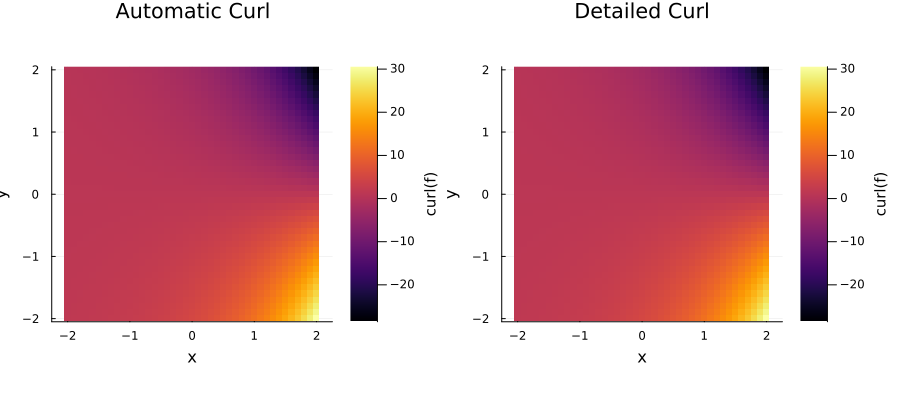
\includegraphics[width=0.5\linewidth]{media/curlcalvsauto-2.png}
        \caption{Plots of  automatic and manual curl calculation.}
        \label{fig:curlcalvsauto-2}
    \end{figure}
\end{solution}

\question  Write a Julia code for the solution of the beam problem shown in Fig. 11. Plot the bending moment diagram (BMD) and shear force diagram (SFD). Your code should be generic enough to take any value for the input variables l and q.
\begin{figure}[H]
    \centering
    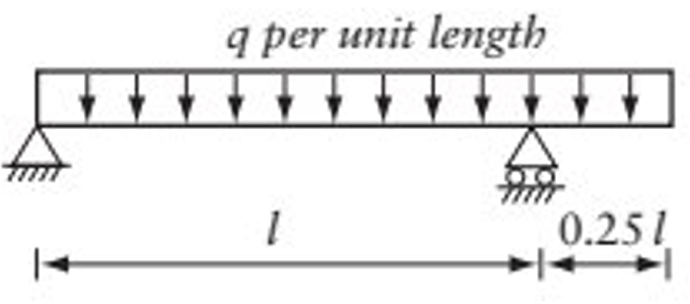
\includegraphics[width=0.4\linewidth]{media/figure-1.png}
    \caption{\empty}
    \label{fig:placeholder}
\end{figure}

\begin{solution}
    \textbf{Solution: 4}
    Plot the bending moment diagram (BMD) and shear force diagram (SFD). 
    \sloppy
    \begin{minted}{julia}
    using Plots 

    # --- Input variables ---
    # Define the total length of the beam (l) and the uniform load (q).
    l = 10.0   # Length of the main span in meters
    q = 5.0    # Uniform distributed load in N/m
    
    # --- Calculations ---
    R_B = (1.25-(1.25^2)/2) * q * l
    R_A = 1.25 * q * l - R_B
    
    # 2. Define the functions for shear force (V) and bending moment (M) along the beam.
    # x is the position along the beam, from 0 to 1.25l.
    function shear_force(x, q, R_A, R_B)
        if x <= l  # Section from left support to right support (0 <= x <= l)
            return R_A - q * x
        else
            # Section on the overhang (l < x <= 1.25l)
            return R_A + R_B - q * x
        end
    end
    
    function bending_moment(x, q, R_A, R_B)
        if x <= l   # Section from left support to right support (0 <= x <= l)
            return R_A * x - (q * x * x) / 2
        else
            # Section on the overhang (l < x <= 1.25l)
            # Let x' be the distance from the right end (x' = 1.25l - x).
            # M = -q * x'^2 / 2
            x_prime = (1.25 * l) - x
            return - (q * x_prime * x_prime) / 2
        end
    end  

    # --- Plotting ---
    # Create an array of x-values for the plot.
    x_values = range(0, stop=1.25*l, length=100)
    \end{minted}
    \begin{minted}{julia}
    # Calculate the corresponding shear force and bending moment values.
    V_values = [shear_force(x, q, R_A, R_B) for x in x_values]
    M_values = [bending_moment(x, q, R_A, R_B) for x in x_values]
    
    # Plot the Shear Force Diagram (SFD).
    sfd_plot = plot(x_values, V_values, title="Shear Force Diagram", xlabel="Position along beam (m)", ylabel="Shear Force (N)", label="", lw=2, linecolor=:blue, grid=true, size=(800, 400))
    hline!([0], lw=1, linecolor=:black, linestyle=:dash)
    
    # Plot the Bending Moment Diagram (BMD).
    bmd_plot = plot(x_values, M_values, title="Bending Moment Diagram", xlabel="Position along beam (m)", ylabel="Bending Moment (N.m)", label="", lw=2, linecolor=:red, grid=true, size=(800, 400))
    hline!([0], lw=1, linecolor=:black, linestyle=:dash)
    
    # Display the plots.
    plot(sfd_plot, bmd_plot)
    \end{minted}
    
    \begin{itemize}
        \item Output $\rightarrow$ Figure -~\ref{fig:sbd-bmd-1}
    \end{itemize}
    
    \begin{figure}[H]
        \centering
        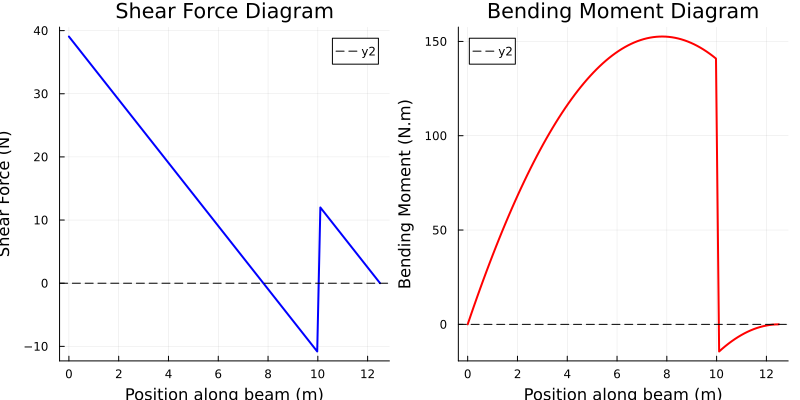
\includegraphics[width=0.5\linewidth]{media/sbd-bmd-1.png}
        \caption{SFD and BMD diagram}
        \label{fig:sbd-bmd-1}
    \end{figure}   
\end{solution}

\question  Write a Julia code for the solution of the beam problem shown in Fig. 13. Plot the BMD and SFD. Your code should be generic enough to take any value for the input variables l and q.
\begin{figure}[H]
    \centering
    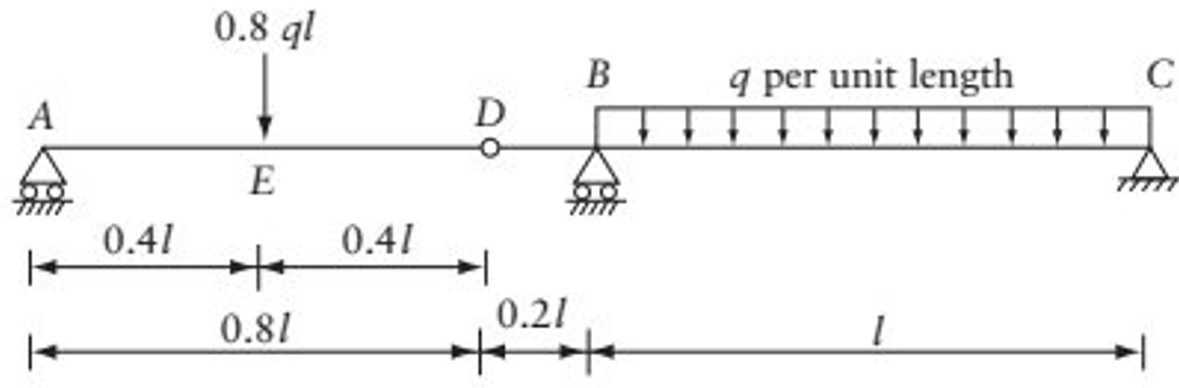
\includegraphics[width=0.5\linewidth]{media/figure-2.png}
    \caption{\empty}
    \label{fig:figure-2}
\end{figure}

\begin{solution}
    \textbf{Solution: 5}
    Plot the bending moment diagram (BMD) and shear force diagram (SFD). 
    \begin{minted}{julia}
    using Plots

    # --- Input variables ---
    # Define the total length of the main span (l) and the uniform load (q).
    l = 10.0   # Length parameter in meters.
    q = 5.0    # Uniform distributed load in N/m

    # --- Calculations ---
    R_A = 0.4 * q * l
    R_B = 0.98 * q * l 
    R_C = 1.8 * q * l - R_A - R_B

    # --- Define Shear Force and Bending Moment Functions ---
    # These functions calculate the internal forces at any point 'x' along the beam.
    # The beam is divided into four sections based on the loads and supports.
    function shear_force(x, l, q, R_A, R_B)
        if x <= 0.4l  # Section AE (0 <= x <= 0.4l)
            return R_A
        elseif x <= 0.8l  # Section ED (0.4l < x <= 0.8l)
            return R_A - (0.8 * q * l)
        elseif x <= l  # Section DB (0.8l < x <= l)
            return R_A - (0.8 * q * l)
        else
            # Section BC (l < x <= 2l)
            return R_A - (0.8 * q * l) + R_B - q * (x - l)
        end
    end
    function bending_moment(x, l, q, R_A, R_B)
        if x <= 0.4l # Section AE (0 <= x <= 0.4l)
            return R_A * x
        elseif x <= 0.8l # Section ED (0.4l < x <= 0.8l)
            return R_A * x - (0.8 * q * l) * (x - 0.4l)
        elseif x <= l  # Section DB (0.8l < x <= l)
            return R_A * x - (0.8 * q * l) * (x - 0.4l)
        else
            # Section BC (l < x <= 2l)
            return R_A * x - (0.8 * q * l) * (x - 0.4l) + R_B * (x - l) - (q * (x - l)^2) / 2
        end
    end
    \end{minted}
    \begin{minted}{julia}
    # --- Plotting ---
    # Define range of x
    x_values = range(0, stop=2l, length=200)
    
    # Calculate the corresponding shear force and bending moment values.
    V_values = [shear_force(x, l, q, R_A, R_B) for x in x_values]
    M_values = [bending_moment(x, l, q, R_A, R_B) for x in x_values]
    
    # Plot the Shear Force Diagram (SFD).
    sfd_plot = plot(x_values, V_values, title="Shear Force Diagram", xlabel="Position along beam (m)", ylabel="Shear Force (N)", label="", lw=2, linecolor=:blue, grid=true, size=(800, 400))
    hline!([0], lw=1, linecolor=:black, linestyle=:dash);
    
    # Plot the Bending Moment Diagram (BMD).
    bmd_plot = plot(x_values, M_values, title="Bending Moment Diagram", xlabel="Position along beam (m)", ylabel="Bending Moment (N.m)", label="", lw=2, linecolor=:red, grid=true, size=(800, 400))
    hline!([0], lw=1, linecolor=:black, linestyle=:dash);
    
    # Display the plots.
    plot(sfd_plot, bmd_plot)
    \end{minted}
    
    \begin{figure}[H]
        \centering
        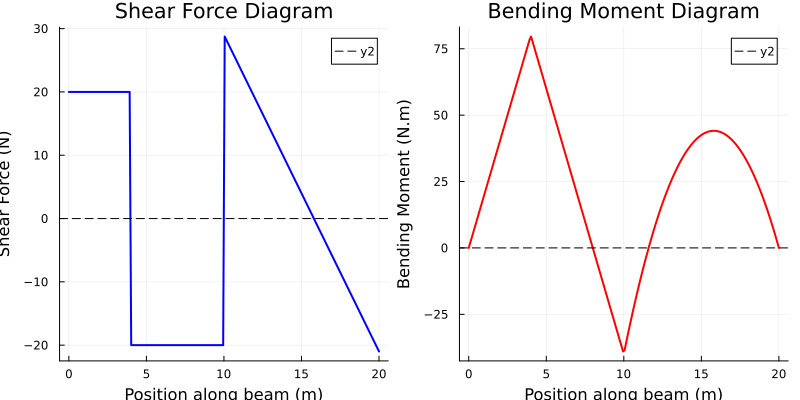
\includegraphics[width=0.5\linewidth]{media/sbd-bmd-2.png}
        \caption{SFD and BMD diagram}
        \label{fig:this}
    \end{figure}
\end{solution}


% citations
% \bibliographystyle{plain}
% \bibliography{citations.bib}

\vspace{2cm}  % Adds vertical space before the ending line
\begin{center}
    \textbf{-- -- -- The End -- -- --}
\end{center}

\end{document}
